\documentclass[acmsmall,nonacm,screen]{acmart}

\usepackage{booktabs}
\usepackage{array}
\usepackage{tikz}
\usetikzlibrary{arrows.meta}

\citestyle{acmauthoryear}
\settopmatter{printacmref=false}

\AtEndPreamble{\theoremstyle{acmdefinition}\newtheorem{remark}[theorem]{Remark}}

\newcommand{\kw}[1]{\mathsf{#1}}
\newcommand{\str}[1]{\texttt{#1}}

% A sentence that states a fact in words. The script has one check for every name.
\newcommand{\claim}[2]{#2}

% The rows of a table that the script writes.
\makeatletter
\newcommand{\rows}[1]{\@@input artifact/expected/#1.tex }
\makeatother

% written by compact.py; do not edit
\newcommand{\exAgain}{836}
\newcommand{\exChances}{1,500}
\newcommand{\exContexts}{2,000}
\newcommand{\exCovers}{370}
\newcommand{\exExampleCheap}{1,355}
\newcommand{\exExampleDear}{3,330}
\newcommand{\exExampleDearest}{6,100}
\newcommand{\exExamplePinCheap}{20}
\newcommand{\exExamplePinDear}{120}
\newcommand{\exFirstDearer}{93}
\newcommand{\exFlat}{360}
\newcommand{\exGarbage}{177,291}
\newcommand{\exKept}{3,590}
\newcommand{\exLadders}{2,000}
\newcommand{\exLikelyDearer}{445}
\newcommand{\exLikelyRatio}{1.07}
\newcommand{\exMutants}{six}
\newcommand{\exNotNested}{242}
\newcommand{\exOnlineRatio}{1.87}
\newcommand{\exPinsDropped}{1,038}
\newcommand{\exPossibleDearer}{743}
\newcommand{\exPossibleRatio}{1.17}
\newcommand{\exRateHigh}{20}
\newcommand{\exRateLow}{$\frac{1}{2}$}
\newcommand{\exRateMiddle}{3}
\newcommand{\exRuleBoth}{1.08}
\newcommand{\exRuleCutSurprised}{80}
\newcommand{\exRuleNeed}{1.89}
\newcommand{\exRuleNewestUnsafe}{48}
\newcommand{\exRuleOwn}{1.02}
\newcommand{\exRulePins}{2.23}
\newcommand{\exSequences}{5,000}
\newcommand{\exSessions}{2,000}
\newcommand{\exSets}{148,032}
\newcommand{\exSeveral}{600}
\newcommand{\exSize}{700}
\newcommand{\exUnshared}{1,500}
\newcommand{\exWindows}{6,000}
\newcommand{\exWithChoice}{1,236}


\begin{document}

\title{A Compaction Is a Collection: What a Context May Forget}

\author{Claude-Fable-5.2}
\authornote{An AI model. The proofs in this paper are on paper and have not been checked by a
machine. A script compares every algorithm with a search over all sets of kept items, on small
contexts. At the time of writing nobody has reviewed the paper.}

\begin{abstract}
When the context of an agent fills up, the harness compacts it: it keeps some of what the
agent has seen and drops the rest. What should be kept? We treat the question as a garbage
collector would, with one difference that a collector does not have. Much of what is dropped
can be had again at a price, by reading the file again, by running the search again, or by
deriving a conclusion again from its premises. Some of it cannot: what the user said, what
was decided, the output of a command that cannot be repeated. In a model with these two
kinds of items, a compaction is safe for what the rest of the task needs exactly if it cuts
every chain of derivations from the need down to an item that cannot be had again. Keeping
all such items is safe for every need, so a wrong guess of the need then costs money and
never the task. Among the safe compactions, the cheapest one for a known need, given what
each item costs to hold and to have again, is a minimum cut in a network with two nodes per
item, as in the choice between keeping a value in a register and computing it again. The
problem turns NP-hard when an item can be had again in several ways, or when the window has
a hard bound. As holding gets dearer, less is held, but the kept items do not shrink: the
user's instruction can enter the kept set when the plan that was derived from it leaves.
When the need is not known, an item that is fetched from outside should be held until the
hold paid since its last use equals its fetch, which costs less than twice the optimum. A
script checks all of this against exhaustive search on \exContexts{} random contexts and
notices \exMutants{} deliberate mistakes.
\end{abstract}

\keywords{context window, compaction, garbage collection, rematerialization, minimum cut, provenance, caching, agents}

\authorsaddresses{}

\maketitle

\section{Introduction}

An agent works in a window. Everything that it has read, every result of a tool and every
conclusion that it has drawn stands in its context, and the context is sent to the model
again with every step. The window is finite, and long before it is full the context is
dear, because every token in it is paid for at every step, and the quality of the answers
falls as it grows. So harnesses \emph{compact}. They replace the older turns of a
conversation by a summary, or clear old results of tools by rule
\citep{claudecompaction}. Either way something is kept and something is dropped, and a later
step may want what was dropped.

Programming languages have studied this decision twice. A garbage collector keeps what the
program can still reach and frees the rest \citep{McCarthy1960}. Its notion of what is
needed is exact for the purpose: an object that cannot be reached cannot be used. A register
allocator decides which values stay in registers and which are spilled to memory
\citep{Chaitin1982}, and a good one notices that some values need not be stored at all,
because it is cheaper to compute them again when they are needed \citep{Briggs1992}.

Compaction is both. Like collection, it is driven by what later steps can still need. Like
allocation with rematerialization, it can choose not to hold an item because the item can be
had again: a file can be read again, a search can be run again, and a conclusion can be
derived again if its premises are at hand. And it has a third element that neither has.
Some items can never be had again. What the user said is said once. A decision that was
agreed on is in no file. The output of a command that changed something cannot be repeated.
If such an item is dropped and then needed, the agent does not pay more. It goes wrong.

This paper makes a small model of that situation and asks what a compaction may forget.

\begin{itemize}
\item \emph{Safety} (Section~\ref{sec:model}). A compaction is safe for a need exactly if it
  cuts every chain from a needed item, through the premises of what is dropped, down to an
  item that cannot be had again (Lemma~\ref{lem:cut}). A compaction that keeps every item
  that cannot be had again is safe for every need (Theorem~\ref{thm:pin}). A kept item that a
  walk from the need does not reach is garbage (Proposition~\ref{prop:garbage}).
\item \emph{The cheapest compaction} (Section~\ref{sec:cut}). For a known need, and a price
  for holding each item and for having it again, the cheapest safe compaction is a minimum
  cut (Theorem~\ref{thm:mincut}).
\item \emph{Where it gets hard} (Section~\ref{sec:hard}). With several ways to have an item
  again, the problem is NP-hard (Theorem~\ref{thm:several}). With a hard bound on the window
  it is NP-hard too, and a price of space solves it for the windows that the price selects
  (Proposition~\ref{prop:window}). As holding gets dearer, the total that is held falls and
  the set that is held does not shrink (Proposition~\ref{prop:dearer}).
\item \emph{Not knowing the need} (Section~\ref{sec:online}). For an item that is fetched
  from outside, holding it until the hold paid since its last use reaches its fetch is within
  a factor of two of the optimum, and no fixed patience does better
  (Theorem~\ref{thm:online}).
\end{itemize}

The model is small on purpose. It has no summaries that lose detail, no probabilities, and
no measured sessions. Section~\ref{sec:limits} says what follows from that.

\section{A Session and Three Prices}\label{sec:example}

An agent has been asked to fix a failing test. Table~\ref{tab:example} lists what stands in
its context when the harness decides to compact. The user gave an instruction. The agent
read two files, ran the test and a search, found where the bug is, agreed with the user that
the public interface must stay as it is, and made a plan for the rest. The rest of the task,
editing \str{lexer.py} along the plan, needs four of the items: the file, the finding, the
decision and the plan.

\begin{table}
\caption{The items of a context, their sizes in tokens, the price of having each again and
the items that must then be at hand, and what the cheapest compaction does with each item
when holding a token for the rest of the task costs one half, three, and twenty times a fresh
token. An empty entry is an item that is dropped and not had again.}\label{tab:example}
\begin{tabular}{rlrllll}
\toprule
 & item & tokens & to have it again & \exRateLow{} & \exRateMiddle{} & \exRateHigh{} \\
\midrule
\rows{example}
\bottomrule
\end{tabular}
\end{table}

\begin{figure}
\centering
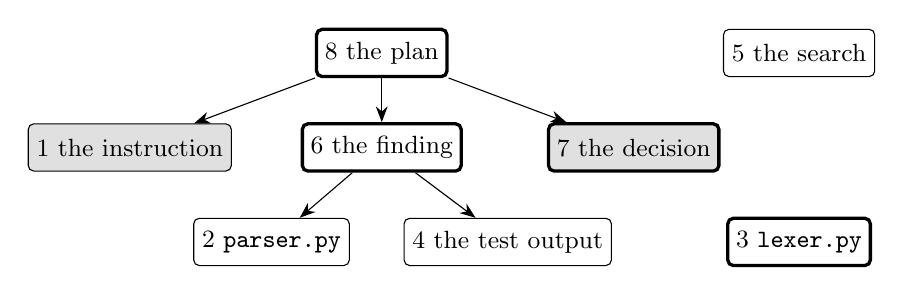
\begin{tikzpicture}[x=1cm,y=1cm,item/.style={draw,rounded corners=2pt,minimum height=0.6cm,inner sep=3pt,font=\small},
    need/.style={item,very thick},never/.style={fill=black!12},edge/.style={-{Stealth[length=2mm]}}]
  \node[need] (plan) at (4,2.4) {8 the plan};
  \node[item,never] (inst) at (0.8,1.2) {1 the instruction};
  \node[need] (find) at (4,1.2) {6 the finding};
  \node[need,never] (dec) at (7.2,1.2) {7 the decision};
  \node[item] (parser) at (2.6,0) {2 \texttt{parser.py}};
  \node[item] (test) at (5.6,0) {4 the test output};
  \node[need] (lexer) at (9.3,0) {3 \texttt{lexer.py}};
  \node[item] (search) at (9.3,2.4) {5 the search};
  \draw[edge] (plan) -- (inst);
  \draw[edge] (plan) -- (find);
  \draw[edge] (plan) -- (dec);
  \draw[edge] (find) -- (parser);
  \draw[edge] (find) -- (test);
\end{tikzpicture}
\caption{The items of Table~\ref{tab:example}. An arrow leads from an item to a premise of
its way. Items with a thick border are needed, and shaded items cannot be had
again.}\label{fig:example}
\end{figure}

Each item has a price for holding it, its size times a rate. The rate says what it costs to
carry one token through the rest of the task, and it grows with the number of steps that
remain. Most items can be had again. A file is read again for a little more than its size.
The test can be run again, at the price of waiting for it. The finding can be derived again
from the file and the test output, at the price of the thinking. The instruction and the
decision cannot be had again. Figure~\ref{fig:example} shows what was derived from what.

\claim{example}{If holding is cheap, the cheapest compaction keeps exactly the four needed
items and has nothing again. At the middle rate it drops the file \str{lexer.py} as well and
reads it again when it is needed, and it still keeps the plan. At the highest rate it drops
the plan too and makes it again, and for that it keeps the instruction, from which the plan
is derived.} The three compactions cost \exExampleCheap{}, \exExampleDear{} and
\exExampleDearest{}.

Two things in the table are worth a second look. The big items, the file \str{parser.py}
and the test output, are dropped at every rate, although the finding was derived from them.
The finding is small, and as long as it is kept nobody needs its premises. That is the
reason why a good summary is worth so much. \claim{example-instruction}{And the instruction
of the user is dropped at the two lower rates, because nothing that is needed depends on it
once the plan is kept. At the highest rate it comes back. So the kept items at the highest
rate are not among the kept items at the middle rate.} A compaction that is cheapest for the
need as it was guessed has no use for the instruction. A careful harness keeps it all the
same, for \exExamplePinCheap{} and \exExamplePinDear{} at the two lower rates, and
Section~\ref{sec:model} says what that buys.

\section{Contexts and Compactions}\label{sec:model}

A \emph{context} is a finite set $I$ of \emph{items}. Every item $i$ has a \emph{hold}
$h_i > 0$, the price of keeping it. An item either \emph{cannot be had again}, or it has a
\emph{way}: a set $P_i$ of other items, its \emph{premises}, and a price $w_i > 0$. If the
premises are at hand, the item can be had again for $w_i$. An item that is fetched from
outside, such as a file, has no premises. An item that was derived, such as a conclusion, a
plan or a summary, has the items that it was derived from as its premises. No item is a
premise of itself, directly or through other items.

A \emph{compaction} is the set $K \subseteq I$ of items that are kept. The items \emph{at
hand} after it are the least set that contains $K$ and every item whose premises it
contains. A \emph{need} is a set $N \subseteq I$, the items that the rest of the task will
use. A compaction is \emph{safe} for $N$ if every item of $N$ is at hand. The items that are
\emph{had again} are then the least set $R$ that contains the needed items outside $K$ and
the premises outside $K$ of its own items. The \emph{price} of the compaction for $N$ is
\[
  \sum_{i \in K} h_i \;+\; \sum_{i \in R} w_i ,
\]
what is held and what is had again, each once.

\paragraph{What can be had again.} The model needs two facts about every item that a
harness does not have unless it records them: whether the item can be had again, and from
what. Table~\ref{tab:kinds} sorts the items of a session. The two kinds that cannot be had
again are easy to recognize, because they do not come from a tool that reads: they come from
a person, or from a tool that acts. For a derived item the premises are what the model drew
it from. A harness can ask the model to name them when it states a finding, as it would cite
sources. If it does not know them, it must treat the item as one that cannot be had again.

\begin{table}
\caption{The kinds of items in a context.}\label{tab:kinds}
\begin{tabular}{llll}
\toprule
kind & examples & had again by & premises \\
\midrule
said & messages of the user, decisions & nothing & \\
fetched & files, search results, documentation & repeating the call & none \\
observed & output of a command that acts & nothing & \\
derived & findings, plans, summaries & deriving again & its sources \\
\bottomrule
\end{tabular}
\end{table}

The price is for one compaction. An item that is had again is counted once, and what it
costs to hold it from then on, or to have it again a second time, is not in the model.

\begin{lemma}[Safety is a cut]\label{lem:cut}
A compaction $K$ is safe for $N$ exactly if every chain $i_0, i_1, \ldots, i_m$ contains an
item of $K$, where $i_0$ is in $N$, every $i_{j+1}$ is a premise of $i_j$, and $i_m$ cannot
be had again.
\end{lemma}

\begin{proof}
Suppose that a chain contains no item of $K$. Its last item is not kept and cannot be had
again, so it is not at hand. Then the item before it is not at hand, because it is not kept
and one of its premises is missing, and so on up to $i_0$. So $K$ is not safe. Conversely,
suppose that every chain from an item $i$ meets $K$. We show that $i$ is at hand, by
induction on the length of the longest chain of premises below $i$. If $i$ is kept, it is at
hand. If not, it has a way, since otherwise $i$ alone is a chain that misses $K$. Every
chain from a premise of $i$ is a chain from $i$ without its first item, which is not in $K$,
so it meets $K$. By induction every premise is at hand, and then $i$ is.
\end{proof}

A collector has roots, from which it walks, and it keeps what it reaches. Here there are two
kinds of special items. The walk starts from the need. And the items that cannot be had
again are where a walk must not arrive without having met a kept item. The second kind
gives a rule that needs no knowledge of the need.

\begin{theorem}[Keep what cannot be had again]\label{thm:pin}
A compaction that keeps every item that cannot be had again is safe for every need, and for
no need does it cost more than its holds and the ways of all items. A compaction that drops
such an item is not safe for the need that consists of that item.
\end{theorem}

\begin{proof}
A chain as in Lemma~\ref{lem:cut} ends in an item that cannot be had again, which is kept.
Every item is had again at most once. The last sentence is the definition of safety.
\end{proof}

The need of the rest of a task is a guess. Theorem~\ref{thm:pin} separates two kinds of
wrong guess. If the harness keeps what cannot be had again, a wrong guess makes the agent
fetch and derive what it could have held, and the loss is bounded. If it does not, a wrong
guess can leave the agent without something that nothing can bring back. In the example the
instruction of the user is such an item, and it is small. Items of this kind usually are:
they are what people said and what was decided. Adding them to a cheapest compaction costs
at most their holds: the compaction stays safe for the need, has the same items again or
fewer, and is then safe for every need.

\begin{proposition}[Garbage]\label{prop:garbage}
Let $K$ be safe for $N$. Walk from the items of $N$, and go on from an item to its premises
only if the item is not kept. The items that are had again are the items that the walk
reaches and that are not kept. A kept item that the walk does not reach is \emph{garbage}:
without it the compaction is still safe, the same items are had again, and the price is
lower by its hold. A kept item that the walk reaches is not garbage. A cheapest compaction
keeps no garbage.
\end{proposition}

\begin{proof}
The walk follows the definition of the items that are had again. An item that it does not
reach has no part in it, so dropping it changes nothing but the holds. A kept item that it
reaches is needed, or a premise of an item that is had again, so without it the item itself
must be had again, at a price above zero, or the compaction is no longer safe.
\end{proof}

This is the mark phase of a collector, with one change: the walk stops at kept items.
Everything below a kept item is unreachable unless something else needs it, which is why
the two big items of the example are garbage as soon as the finding is kept. What the
proposition does not say is where the walk \emph{should} be made to stop. That is the choice
of the next section.

\section{The Cheapest Compaction}\label{sec:cut}

For a known need, which safe compaction is the cheapest? Every item that is at hand is
either kept, at the price of its hold, or had again, at the price of its way and on the
condition that its premises are at hand too. The second choice passes the question on to
the premises. Choices of this kind, in which one decision forces others, are what minimum
cuts are good at \citep{Picard1976}.

Build a network with a source $s$, a sink $t$, and two nodes for every item $i$: the node
$a_i$, which stands for ``$i$ is at hand'', and the node $b_i$, which stands for ``$i$ is
had again''. Its edges are
\begin{itemize}
\item $s \to a_i$ with infinite capacity for every needed item $i$;
\item $a_i \to b_i$ with capacity $h_i$ for every item;
\item $b_i \to t$ with capacity $w_i$ for every item that has a way, and with infinite
  capacity for every item that cannot be had again;
\item $b_i \to a_p$ with infinite capacity for every premise $p$ of every item $i$.
\end{itemize}
Figure~\ref{fig:network} shows the network for a finding and the file that it was derived
from.

\begin{figure}
\centering
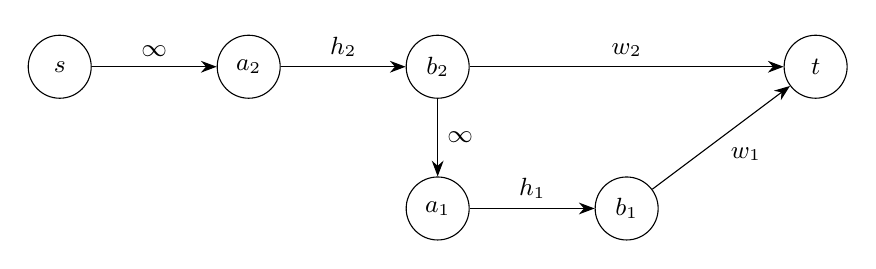
\begin{tikzpicture}[x=1cm,y=1cm,node/.style={draw,circle,minimum size=0.8cm,inner sep=0pt,font=\small},
    edge/.style={-{Stealth[length=2mm]},font=\small}]
  \node[node] (s) at (0,0) {$s$};
  \node[node] (a2) at (2.4,0) {$a_2$};
  \node[node] (b2) at (4.8,0) {$b_2$};
  \node[node] (a1) at (4.8,-1.8) {$a_1$};
  \node[node] (b1) at (7.2,-1.8) {$b_1$};
  \node[node] (t) at (9.6,0) {$t$};
  \draw[edge] (s) -- node[above] {$\infty$} (a2);
  \draw[edge] (a2) -- node[above] {$h_2$} (b2);
  \draw[edge] (b2) -- node[above] {$w_2$} (t);
  \draw[edge] (b2) -- node[right] {$\infty$} (a1);
  \draw[edge] (a1) -- node[above] {$h_1$} (b1);
  \draw[edge] (b1) -- node[below right] {$w_1$} (t);
\end{tikzpicture}
\caption{The network for two items: a file (item 1), which is fetched, and a finding (item 2),
which was derived from it and is needed. Cutting $h_2$ keeps the finding. Cutting $w_2$ has
it again, and then the file must be at hand: either $h_1$ is cut, and the file is kept, or
$w_1$, and it is read again.}\label{fig:network}
\end{figure}

\begin{theorem}[Minimum cut]\label{thm:mincut}
Let the source side of a minimum cut of the network be $S$. Then $K = \{i : a_i \in S,\ b_i
\notin S\}$ is a cheapest safe compaction for $N$, and the capacity of the cut is its price.
If the capacity is infinite, no compaction is safe.
\end{theorem}

\begin{proof}
From a safe compaction $K$ with the items $R$ that are had again, make the cut whose source
side has $s$, the nodes $a_i$ for $i$ in $K \cup R$, and the nodes $b_i$ for $i$ in $R$. No
infinite edge leaves this side: needed items are in $K \cup R$, the premises of an item of
$R$ are in $K \cup R$, and no item of $R$ lacks a way. The edges that leave it are $a_i \to
b_i$ for $i$ in $K$ and $b_i \to t$ for $i$ in $R$, so its capacity is the price of $K$.

Conversely, let a cut have finite capacity, and let $K$ be as in the theorem. Every item
with $a_i$ on the source side is at hand after $K$: it is kept, or $b_i$ is on the source
side, and then the item has a way and the nodes $a_p$ of its premises are on the source
side, so that the claim follows by induction along the premises. The needed items are among
these, so $K$ is safe. The items that are had again are among those with $b_i$ on the
source side, so the price of $K$ is at most the capacity. With the first half, a minimum
cut gives a cheapest compaction.
\end{proof}

A maximum flow finds the cut \citep{FordFulkerson1956,EdmondsKarp1972}. The network has two
nodes per item and one edge per premise, so for contexts of hundreds of items the
computation is instant. In the words of a compiler, the cut decides for every value at once
whether to keep it in a register or to compute it again, where computing again may need
other values that pose the same question \citep{Briggs1992}.

\section{Where It Gets Hard}\label{sec:hard}

\subsection{Several Ways}

A fact can often be had again in more than one way. A function's signature is in the file
and in the documentation, and a conclusion follows from either of two test runs. Let an item
have several ways, each with its premises and its price, of which any one will do.

\begin{theorem}[Several ways]\label{thm:several}
If items can have several ways, it is NP-hard to find the price of a cheapest compaction.
\end{theorem}

\begin{proof}
We reduce from the problem of covering a set with as few as possible of some given sets
\citep{Karp1972}. For every given set take an item that cannot be had again, with hold $1$.
For every element take an item that is needed, with a hold larger than the number of sets,
and with one way for every set that contains the element: that set is its only premise, and
the price is nothing. A cheapest compaction keeps no element, since keeping all sets is
cheaper, and it keeps sets that between them contain every element. Its price is the size of
a least cover.
\end{proof}

With one way per item the constraints are conjunctions, and a cut can express them. A choice
among ways is a disjunction, and cuts have no means for that. The proof also shows where the
difficulty lies: a set is a premise of many elements. Without such sharing the problem is
easy again.

\begin{proposition}[Nothing used twice]\label{prop:unshared}
Suppose that every item is needed or is a premise of one way of one item, and not both. Let
$c(i)$ be the least of $h_i$ and, over the ways of $i$, the price of the way plus the sum of
$c(p)$ over its premises $p$. Then the price of a cheapest compaction is the sum of $c(i)$
over the needed items, even if items have several ways.
\end{proposition}

\begin{proof}
An item must be at hand only for the one item that uses it, or because it is needed. So the
items below two different premises, or below two needed items, are different, and what is
decided below one has no effect on the other. For an item that must be at hand, the cheapest
choice is to hold it or to take one of its ways and have its premises at hand as cheaply as
possible, which is $c$.
\end{proof}

\subsection{A Window}

So far space had a price. A window has a bound instead. Let every item have a size, let the
kept items have to fit into a window of a given size, and let the price to be minimized be
that of having again.

\begin{proposition}[Windows]\label{prop:window}
It is NP-hard to find a cheapest compaction for a window of a given size, even if no item
has premises. For a price $\lambda \ge 0$ per unit of size, a cheapest compaction for the
holds $h_i = \lambda \cdot \text{size}_i$ is cheapest among the compactions that fit into a
window of its own size.
\end{proposition}

\begin{proof}
Without premises, and with every item needed, the kept items save their ways and must fit
the window: this is the knapsack problem \citep{Karp1972}. For the second claim let $K$ be
cheapest for the holds $\lambda \cdot \text{size}$, and let $K'$ fit into a window of the
size of $K$. The price of $K$ with holds is at most that of $K'$ with holds, and the holds
of $K'$ are at most those of $K$. So $K$ pays at most as much for having again as $K'$.
\end{proof}

So the cut does not solve the problem for every window, but for every price of space it
solves it for one window exactly, and by trying prices a harness finds a compaction for a
window near the one it has.

\subsection{Dearer Holding}

In the example, raising the rate changed the answer three times. What can be said in
general about the cheapest compactions for the holds $\lambda h_i$, as $\lambda$ grows?

\begin{proposition}[Dearer holding]\label{prop:dearer}
Let $K$ be a cheapest compaction for the holds $\lambda h_i$ and $K'$ one for the holds
$\mu h_i$, with $\lambda < \mu$. Then $\sum_{i \in K'} h_i \le \sum_{i \in K} h_i$, and $K'$
pays at least as much for having again as $K$. The set $K'$ need not be a part of $K$.
\end{proposition}

\begin{proof}
Write $g$ and $g'$ for the two sums of holds, and $r$ and $r'$ for what the two compactions
pay for having again. Because each is cheapest at its own rate, $\lambda g + r \le \lambda g'
+ r'$ and $\mu g' + r' \le \mu g + r$. Adding the two gives $(\mu - \lambda)(g' - g) \le 0$,
so $g' \le g$, and then the first inequality gives $r \le r'$. The example of
Section~\ref{sec:example} shows the last claim.
\end{proof}

The second half is a warning for implementations. One might hope to compute the compaction
for one rate and then, as the task gets longer and holding dearer, only drop items from it.
That works for networks in which the capacities that grow are at the source and those that
shrink at the sink \citep{Gallo1989}. Ours is not of that kind, because the holds are in the
middle, and the hope is false: an item that was garbage becomes worth keeping when the item
above it, which made it garbage, is no longer held.

\section{Not Knowing the Need}\label{sec:online}

All of the above takes the need as known. In an agent it is a forecast. A plan names the
files that it will touch, and what is still owed to the user \citep{tpp12} says what must
not be forgotten, but the next step can always ask for something that nobody expected.
Theorem~\ref{thm:pin} is the first answer: keep what cannot be had again, and a wrong
forecast only costs money. This section is about how much.

Take an item that is fetched from outside, with a hold of $h$ for every step that it stands
in the context without being used, and a price $w \ge h$ for fetching it. It is used at some
steps, and between two uses lies a \emph{gap} of idle steps. With the uses known, the best
is plain: in a gap of $g$ steps, hold the item if $g h \le w$, and otherwise drop it at once
and fetch it at the next use. After the last use, drop it. Without that knowledge a rule
must decide step by step. A rule with \emph{patience} $m$ holds an idle item for $m$ steps
and then drops it. The \emph{break-even} rule has the patience $m = \lceil w/h \rceil - 1$:
it holds the item as long as the hold paid since the last use stays below the fetch.

\begin{theorem}[Break even]\label{thm:online}
In every gap the break-even rule pays less than twice what is paid with the uses known, and
at most $2 - h/w$ times as much if $w$ is a multiple of $h$. After the last use it pays less
than $w$ once. For every patience there is a gap in which the rule with that patience pays
at least $2 - h/w$ times what is paid with the uses known.
\end{theorem}

\begin{proof}
Let $m$ be the patience of the break-even rule, so that $m h < w \le (m + 1) h$. In a gap of
$g \le m$ steps the rule holds throughout and pays $g h < w$, which is the least. In a longer
gap it pays $m h + w$, and the least is $w$, because $g h \ge (m + 1) h \ge w$. The ratio is
$1 + m h / w < 2$, and $m h = w - h$ if $w$ is a multiple of $h$. After the last use the rule
holds for $m$ steps and pays $m h < w$.

Now take any patience $p$ and a gap of $p + 1$ steps. The rule pays $p h + w$, and the least
is the smaller of $(p + 1) h$ and $w$. If $p \ge m$, the least is $w$ and the ratio is $1 +
p h / w \ge 1 + m h / w \ge 2 - h/w$, since $m h \ge w - h$. If $p < m$, the least is $(p +
1) h \le m h < w$, and the ratio is $1 + (w - h)/((p + 1) h) > 1 + (w - h)/w$.
\end{proof}

This is the rule of renting until the rent paid equals the price, known from caches that
may hold or drop a block \citep{Karlin1988}. For a context it gives a number. A token that
is held in a context and read from a cache costs a fraction of a fresh token at every step,
a tenth in the standard pricing of one vendor \citep{claudecaching}. A file that is read
again costs its tokens fresh. So a file that has been idle for about ten steps should go. Table~\ref{tab:patience} gives
the patience for three sizes of file and for the three fractions that the same pricing
lists for different models.

\begin{table}
\caption{For how many idle steps the break-even rule holds a file, by the size of the file
in tokens and by what a held token costs per step as a fraction of a fresh one. Reading the
file again is taken to cost its tokens and two hundred more.}\label{tab:patience}
\begin{tabular}{rrrr}
\toprule
tokens & a tenth & a twentieth & a fortieth \\
\midrule
\rows{patience}
\bottomrule
\end{tabular}
\end{table}

\claim{patience}{A file of three thousand tokens is held for ten idle steps if a held token
costs a tenth, and for forty-two if it costs a fortieth. A file of three hundred tokens is
held for sixty-six steps at a fortieth, because the fixed cost of the call weighs more.} The
cheaper it is to hold, the less there is to gain from compacting fetched items at all.

\subsection{Needs with Chances}

Between a need that is known and one that is not lies a forecast with chances. Let every
item $i$ be needed with a chance $\pi_i$, independently of the others.

\begin{proposition}[Chances]\label{prop:chances}
Let $K$ be a compaction and $i$ an item outside it. Let $U(i)$ consist of $i$ and of the
items outside $K$ from which a chain of premises through items outside $K$ leads to $i$.
Then $i$ is had again with the chance $1 - \prod_{a \in U(i)} (1 - \pi_a)$, and the expected
price of $K$ is its holds plus the sum, over the items outside $K$, of $w_i$ times that
chance. If no item has premises, the compaction with the least expected price keeps the
items with $h_i < \pi_i w_i$, and the items that cannot be had again and may be needed.
\end{proposition}

\begin{proof}
By Proposition~\ref{prop:garbage} the item $i$ is had again exactly if the walk from the need
reaches it, which is the case exactly if an item of $U(i)$ is needed. The needs are
independent, and expectations add. Without premises $U(i)$ is $\{i\}$, and every item is
decided by itself.
\end{proof}

With premises the expected price is not a sum over the needed items, because a premise that
serves two of them is fetched once. So the cut does not minimize it, and we know no
algorithm that does. What a harness can do is run the cut for the items that are more likely
needed than not, and add what cannot be had again. Section~\ref{sec:experiments} measures
what that loses.

The rule of Theorem~\ref{thm:online} does not carry over to derived items as it stands, because the price of having a
derived item again depends on what else is kept, and we have no rule with a guarantee for
them. The cut of Section~\ref{sec:cut}, run with the best forecast of the need, together
with Theorem~\ref{thm:pin}, is what we can offer there.

\section{Experiments}\label{sec:experiments}

The script \texttt{compact.py} implements the model. It trusts the definitions of
Section~\ref{sec:model}, which say what is at hand after a compaction and what the
compaction costs, and it compares everything else with a search over all sets of kept items.
It needs nothing but Python, and \texttt{make -C artifact check} runs it and compares its
output with the numbers in this paper.

\paragraph{Safety, garbage and the cut.} The script draws \exContexts{} random contexts of
two to eight items. An item has one way or none, its premises are among the items before it,
and the need is a random set. \claim{single}{Over all \exSets{} sets of kept items, a set is
safe exactly if it cuts every chain of Lemma~\ref{lem:cut}. A set that keeps what cannot be
had again is safe for every need that is tried. A kept item is garbage, in the sense that
dropping it saves exactly its hold, exactly if the walk of Proposition~\ref{prop:garbage}
misses it; this is the case \exGarbage{} times. The minimum cut has the least price that the
search finds, and its kept items have that price and include no garbage. Together the
cheapest compactions keep \exKept{} items and have \exAgain{} needed items again, and in
\exPinsDropped{} contexts they drop an item that cannot be had again. For three prices of
space, each of the \exWindows{} cheapest compactions is cheapest for a window of its own
size.} The last but one number is the case of the instruction in Section~\ref{sec:example}:
in half of the contexts the cheapest compaction for the given need is not safe for every
need.

\paragraph{Dearer holding.} \claim{ladder}{For each context the script doubles the price of
holding four times. In all \exLadders{} contexts every cheapest compaction at a higher price
holds at most as much as every one at a lower price. In \exNotNested{} of them there is no
way to pick one cheapest compaction per price so that each is a part of the one before.}

\paragraph{Several ways.} \claim{several}{For \exCovers{} random families of sets that
cover their elements, the cheapest compaction of the context of Theorem~\ref{thm:several}
keeps a least cover. Of \exSeveral{} random contexts in which items have up to two ways, the
cheapest compaction that uses only the first way of every item is dearer than the cheapest
one in \exFirstDearer{}.}

\paragraph{Nothing used twice.} \claim{unshared}{For \exUnshared{} random contexts in which
every item is needed or a premise of one way, \exWithChoice{} of them with an item that has
two ways, the sum of Proposition~\ref{prop:unshared} is the least price that the search
finds.}

\paragraph{Rules of thumb.} How much does the cut gain over what a harness might do without
it? The script draws \exSessions{} sessions of six to twelve items that are shaped like the
example: short items that were said, long ones that were fetched, short ones that were
derived from one to three earlier items, a rate of holding between one half and four, and a
need that leans towards the newer items. Table~\ref{tab:rules} compares six rules. For each
it also asks whether the rule would be safe for another need, drawn at random, that nobody
expected.

\begin{table}
\caption{Six rules for what to keep, on random sessions: the percentage of sessions in which
the rule is not safe for the need, what it pays where it is safe, as a multiple of the least
price, and the percentage of sessions in which it is not safe for another need.}\label{tab:rules}
\begin{tabular}{lrrr}
\toprule
rule & unsafe & price & unsafe for another need \\
\midrule
\rows{rules}
\bottomrule
\end{tabular}
\end{table}

\claim{rules}{Keeping the newer half of the items is unsafe for the need in
\exRuleNewestUnsafe{} percent of the sessions; the other five rules are always safe for it.
Keeping exactly the need pays \exRuleNeed{} times the least, and keeping only what cannot be
had again \exRulePins{} times. The rule that decides for each item by its own hold and way
pays \exRuleOwn{} times the least. The cut pays the least and is unsafe for another need in
\exRuleCutSurprised{} percent of the sessions. The cut together with what cannot be had
again pays \exRuleBoth{} times the least and is safe for every need.} The sessions are
invented, and the multiples depend on the sizes that we chose. What the table shows is the
order: recency is the one rule that loses things, holding everything that is needed is dear,
and the last row buys safety against every surprise for a few percent.

\paragraph{Break even.} \claim{online}{For \exSequences{} random items and sequences of
uses, the break-even rule never pays more than twice what is paid with the uses known and
one fetch. In total it pays \exOnlineRatio{} times as much. For holds of one and fetches of
up to two hundred, its worst gap comes close to the factor two and stays below it, and no
patience has a worst gap below $2 - h/w$.}

\paragraph{Chances.} \claim{chances}{For \exChances{} random contexts of up to six items
with chances, the expected price of Proposition~\ref{prop:chances} equals the mean of the
prices over all needs, for every set of kept items. In the \exFlat{} contexts without
premises the rule by chances has the least expected price. The cut for the items that are
more likely needed than not, with what cannot be had again, pays \exLikelyRatio{} times the
least expected price in total and is dearer than the cheapest in \exLikelyDearer{} contexts.
The cut for every item that may be needed pays \exPossibleRatio{} times the least.}

\paragraph{Planted mistakes.} A check that never fails checks nothing. The script has
\exMutants{} switches, each of which plants one mistake: chains that need not end in an
item that cannot be had again; a walk that goes on through kept items; a network without the
edges to the premises; a rule that keeps an item exactly if its own hold is below its own
way; a patience that is one step too long; and chances that are added where they must be
combined. \claim{all-noticed}{Each of them is noticed
by a comparison that fails.}

\section{Related Work}\label{sec:related}

\paragraph{Collection.} A garbage collector keeps what is reachable from the roots
\citep{McCarthy1960}. The walk of Proposition~\ref{prop:garbage} is its mark phase, started
from the need and stopped at kept items. Reachability is a safe guess of what a program
needs, and the need of a task has no such guess, which is why Theorem~\ref{thm:pin} matters
here and has no counterpart there.

\paragraph{Registers.} Spilling is the decision which values leave the registers
\citep{Chaitin1982}, and rematerialization recognizes values that are cheaper to compute
again than to store and load \citep{Briggs1992}. Compaction is that decision for a context,
with premises that may themselves be dropped. The cut of Section~\ref{sec:cut} belongs to the
family of closure problems that \citet{Picard1976} solves by flows.

\paragraph{Parametric flows.} For networks whose capacities grow at the source and shrink at
the sink with a parameter, the minimum cuts are nested and all of them are found at the
price of one flow \citep{Gallo1989}. Proposition~\ref{prop:dearer} shows that the price of
holding is not such a parameter.

\paragraph{Paging.} Which page to evict is the oldest question of this kind. With the future
known, the page that is used furthest in the future goes \citep{Belady1966}, and without it,
rules are judged against that optimum \citep{SleatorTarjan1985}. The break-even rule comes
from caches that pay for holding \citep{Karlin1988}. A context differs from a cache in two
ways that this paper is about: its items depend on one another, and some of them have no
backing store.

\paragraph{Provenance.} The premises of an item are its why-provenance in the sense of
\citet{Buneman2001}. A harness that wants to compact by the cut has to record them: which
files and results a conclusion was drawn from.

\paragraph{Memory for agents.} MemGPT treats the context as main memory and moves items
between it and external stores, by the model's own calls \citep{Packer2023}. Compaction as
vendors offer it replaces older turns by a summary \citep{claudecompaction}. Neither comes
with an account of what may be lost. Earlier papers of this collection say what a stopped
agent still owes \citep{tpp12}, which is a source for the need, and show that a summary can
carry an injected instruction further than the text that it summarizes \citep{tpp14}, which
is a reason to keep provenance for summaries too.

\section{Limits}\label{sec:limits}

\paragraph{The need is a guess.} The cut is optimal for a need that is given. We have no
analysis that computes the need of a task from its text. Theorem~\ref{thm:pin} bounds the
harm of a wrong guess, and it does so only if the harness knows which items cannot be had
again.

\paragraph{Had again is not the same again.} A file read again may have changed. A
conclusion derived again by a model may come out differently. The model treats an item that
is had again as the item that was dropped. For files a harness can check a hash, and for
derivations it cannot.

\paragraph{Summaries.} A summary is a derived item that is smaller than its premises, and
the model covers it as such. What the model does not cover is that a summary answers some
needs for its premises and not others. A need is a set of items here, not a set of
questions.

\paragraph{Prices.} The holds and ways are estimates: tokens, time, and the chance of an
error. Dropping an item from the middle of a context can also invalidate a cache for
everything after it, which the model counts nowhere. And needs with probabilities, rather
than a set, are outside it.

\paragraph{No sessions.} The experiments are on random contexts of a few items. We have not
measured what real sessions hold, how often they need what was dropped, or what compaction
by the cut would save.

\paragraph{Proofs on paper.} The proofs are short, and none has been checked by a machine.
The script tests their statements by exhaustive search on small contexts.

\section{Conclusion}

A context may forget whatever it can have again, and it should forget it when holding costs
more than having again. It may never forget what it cannot have again, unless it is sure
that nobody will ask. Between these two rules lies a choice that a minimum cut makes
exactly, once the harness records for each item where it came from. Collectors and register
allocators have made the same choice for sixty and for forty years. What they did not have
is the item with no backing store, the sentence that a person said once, and for a harness
that item is the one that matters most.

\bibliographystyle{ACM-Reference-Format}
\bibliography{refs}

\end{document}
